\section{Question 5}

\subsection{Task}
Seam carving is a special image manipulation. Look it up on Wikipedia to understand what it means. You are free to assumptions to simplify the problem definition as you require. Choose an image that contains two objects of interest separated by large distance and illustrate how your implementation of seam carving works on it.


\subsection{Solution}

Link to the GitHub repository for this question: \href{https://github.com/Xerefic/MM2090-Solutions/tree/master/Final_Assignment/question_5}{GitHub}

\subsubsection{Approach}
We compute the energy of the image using gradient magnitude and find the seam with the minimum energy, a line which is connected to the adjacent pixels either via an edge or a corner. We use dynamic programming to keep track of the minimum seam. \\
The idea is, if we remove the so calculated minimum seam, the image doesn’t lose important features, but we have successfully decreased the dimensions without resizing image.\\
This process can be repeated any number of times, to produce an image of desired dimensions.

\begin{itemize}

	\item \textbf{Computing Energy} \\
The energy is computed by $e_i(I)=\left|\frac{\partial I}{\partial x}\right| + \left|\frac{\partial I}{\partial y}\right|$. \\
Using Sobel Filters, 
$p^{\prime}_u = \begin{bmatrix} +1 & +2 & +1\\ 0 & 0 & 0 \\ -1 & -2 & -1 \end{bmatrix} \circledast I$ and 
$p^{\prime}_v = \begin{bmatrix} +1 & 0 & -1\\ +2 & 0 & -2 \\ +1 & 0 & -1 \end{bmatrix} \circledast I$, we compute the derivative as $e_i(I)=\left|p^{\prime}_u\right| + \left|p^{\prime}_v\right|$.

	\item \textbf{Finding the Seam with least Energy} \\
To compute the seam with the least energy, we dynamically compute $M\left(i,j\right)=e\left(i,j\right)+\min\left( M\left(i-1,j-1\right), M\left(i-1,j\right), M\left(i-1,j+1\right)\right)$ where $M\left(i,j\right)$ stores the minimum energy value stored upto the pixel $\left(i,j\right)$.\\
The minimum energy thus will be stored in the last row of **M** and **backtrack** stores the list of pixels present in this s.

	\item \textbf{Deleting the Minimum Seam} \\
We recursively remove the seam with minimum energy till we reach the image of required size.
\end{itemize}

\subsubsection{Requirements}
Language of choice: python
\begin{lstlisting}[language=bash]
	pip3 install numpy
	pip3 install matplotlib
	pip3 install scipy
\end{lstlisting}

\subsubsection{Observation}
The algorithm is a computationally expensive version to achieve Seam Carving. Since the operations have to be sequential, there is no possibility of using parallel computing realms to speed up the process.\\
NOTE: It took around 25 mins for the first image and over 1 hour for the second image.

\subsubsection{Output}


\begin{table}[!ht]
	\begin{center}
		\begin{tabular}{ | c | c | c | }
			\hline
			ORIGINAL & SEAM CARVED & SCALE \\ \hline
			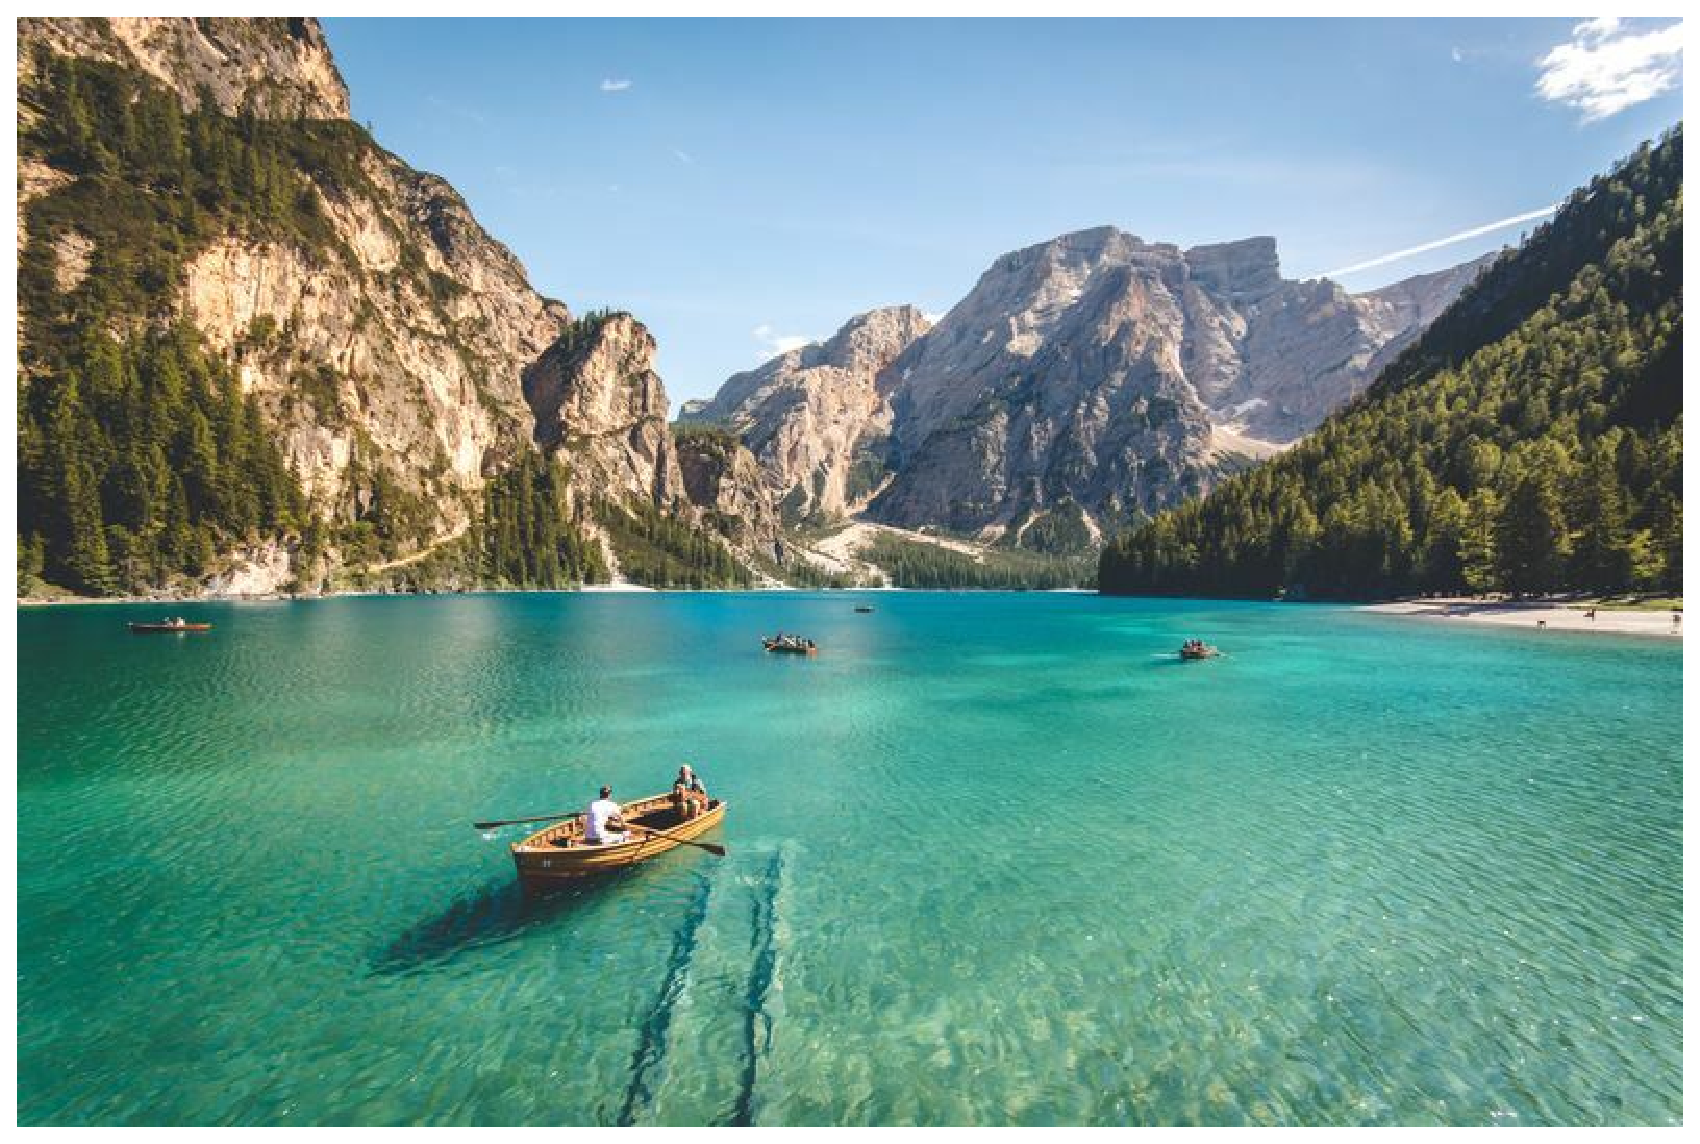
\includegraphics[height=50mm]{question_5/Image-1.eps} & 
			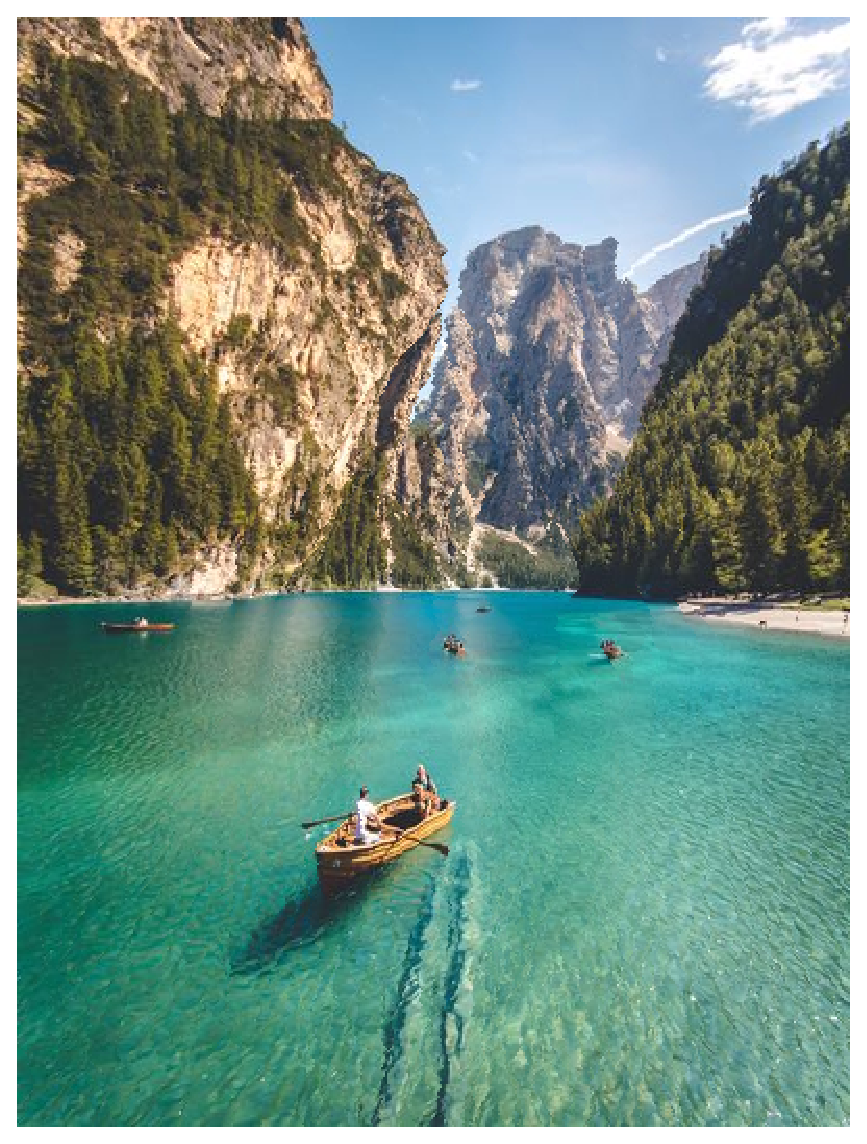
\includegraphics[height=50mm]{question_5/Image-1_scaled_column_by_0.5.eps} & 
				0.5 \\ \hline
			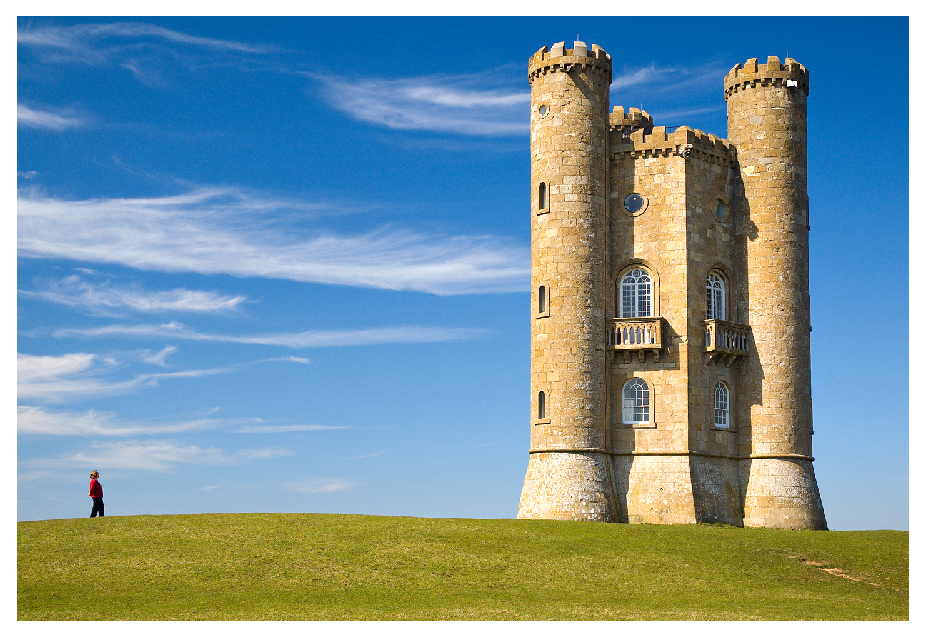
\includegraphics[height=50mm]{question_5/Image-2.eps} & 
			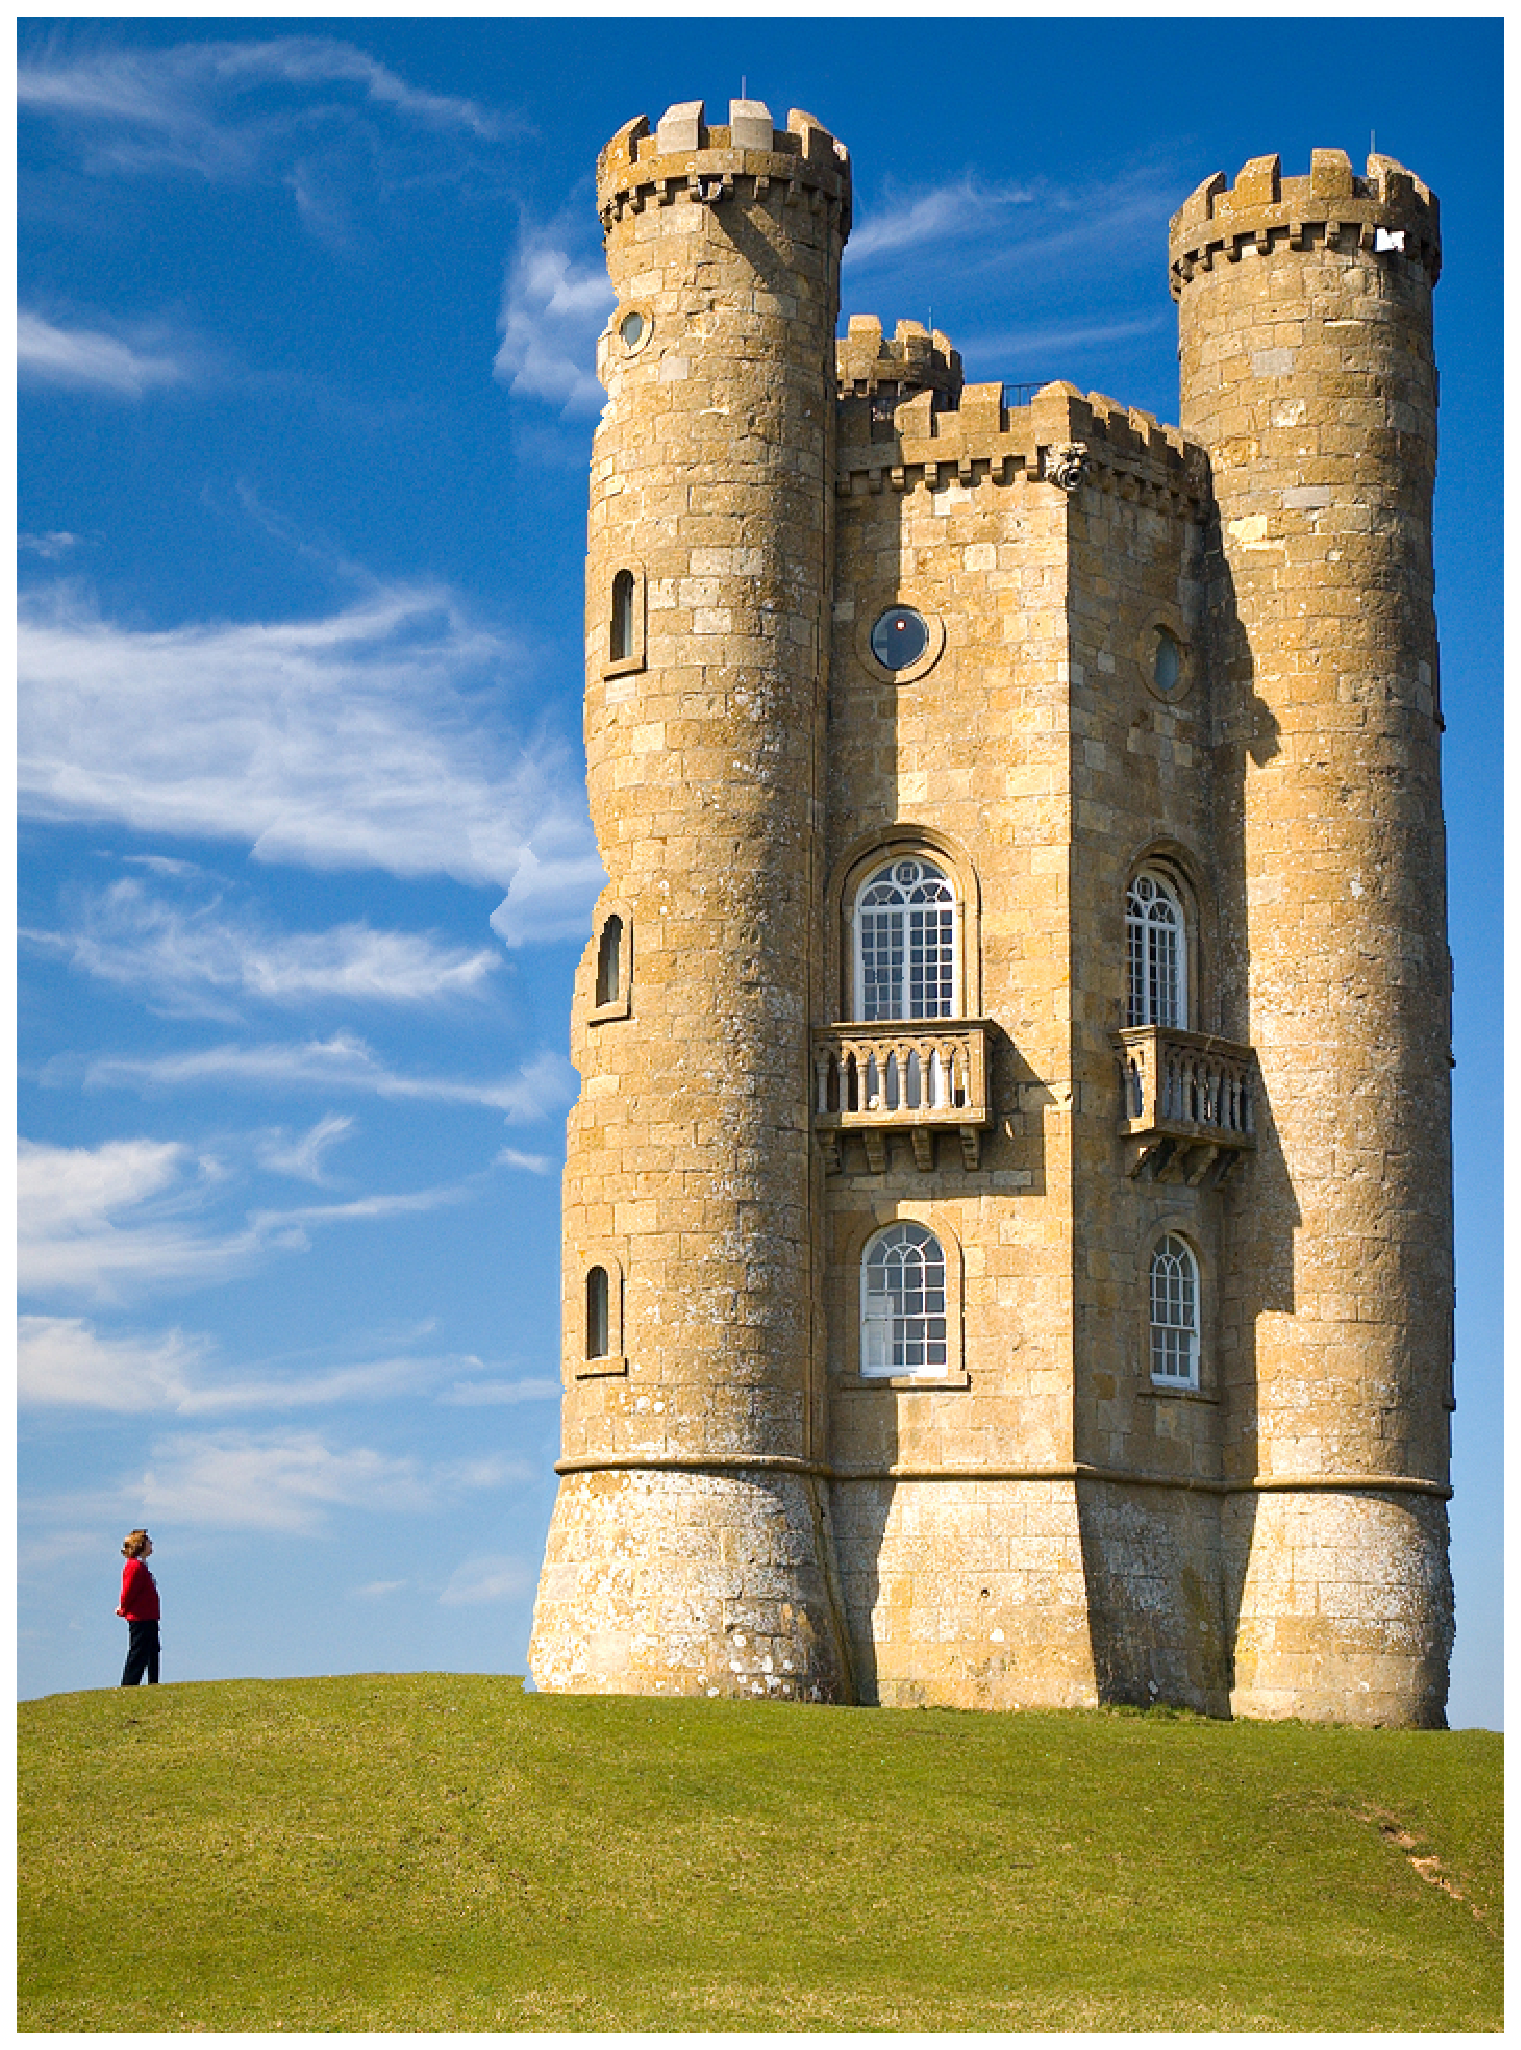
\includegraphics[height=50mm]{question_5/Image-2_scaled_column_by_0.5.eps} & 
				0.5 \\ \hline
		\end{tabular}
	\end{center}
\caption{Processed Images}
\end{table}
